\section{Stepping OCaml in the Classroom}
\label{sec:exp}
Since 2016, we have been using (earlier versions of) our stepper in an
introductory OCaml course called ``Functional Programming'',
taught by the third author at Ochanomizu University.

\subsection{The OCaml Course}
The ``Functional Programming'' course teaches how to program with functions and types, covering
basic topics such as recursion, datatypes, effects, and modules.
The course consists of 15, weekly lab sessions, and each session
 consists of 90 minutes lab-style class per week.
(Many students remain in the lab after 90 minutes up until around 150
minutes.)
Throughout the course, students build a program that searches for
the shortest path based on Dijkstra's algorithm.
The participants of the course are second-year undergraduate students
majoring in computer science (around 40 students each year).
All students enter this course after a CS 1 course in the C
programming language.

The course is taught in a ``flipped classroom'' style.
Before every meeting, students are asked to study assigned readings
and videos prepared by the instructor and answer simple quizzes.
In the classroom, they practice the newly covered topics
through exercises, with assistance of the instructor as well as five
to six teaching assistants (including the first and second authors).  

The exercises include simple practice problems and report problems.
The former are for confirming students' understanding of the
topics and are expected to be completed within a class.
The latter problems (for credit) are due in one week.
Whenever a student executes a program, by either step execution or
standard execution, the program as well as its execution log (syntax
errors, type errors, or the result of execution) are recorded.

For most of the problems (up to the 12th week), we provide a check system
where students can submit their solutions to see whether they pass the
given tests.
To earn points for report problems, students are required to have their
programs pass the check system.

\subsection{The Uses of the Stepper}
We introduced the stepper into Functional Programming in 2016.
Although the steppers used in the past had almost the same user-interface as the one shown in Figure \ref{figure:ocamlfac}, they differ in the following ways:
\begin{description}
\item[2016] This first version supported function definitions,
conditionals, records, lists, and recursion.  However, there were
various operations that were not supported.
As such, the usability of the stepper was low.
Moreover, when the instructor introduced the stepper to students, he
only mildly encouraged to use it.
Although we do not know how much the stepper was used in 2016 since we
did not log the execution of stepper, we expect it was used
only rarely in the first few weeks of the course.
\item[2017] Based on the lessons from the previous year, the second
version supported most operations used in the first six weeks.
The instructor introduced the stepper up front at the first class and
showed how to use the stepper with various examples in the subsequent
classes.
\item[2018] The third version supported almost all the constructs
needed for the course, including modules, exception handling,
sequential execution, printing, references, and arrays.
It also supported skipping of function application.
The instructor introduced the stepper as though the stepper was the
only way to execute OCaml programs, encouraging the uses of the
stepper.
(Students gradually realized that they could execute a program in the
interpreter in a few weeks.)
\end{description}

\begin{figure}
  \begin{center}
    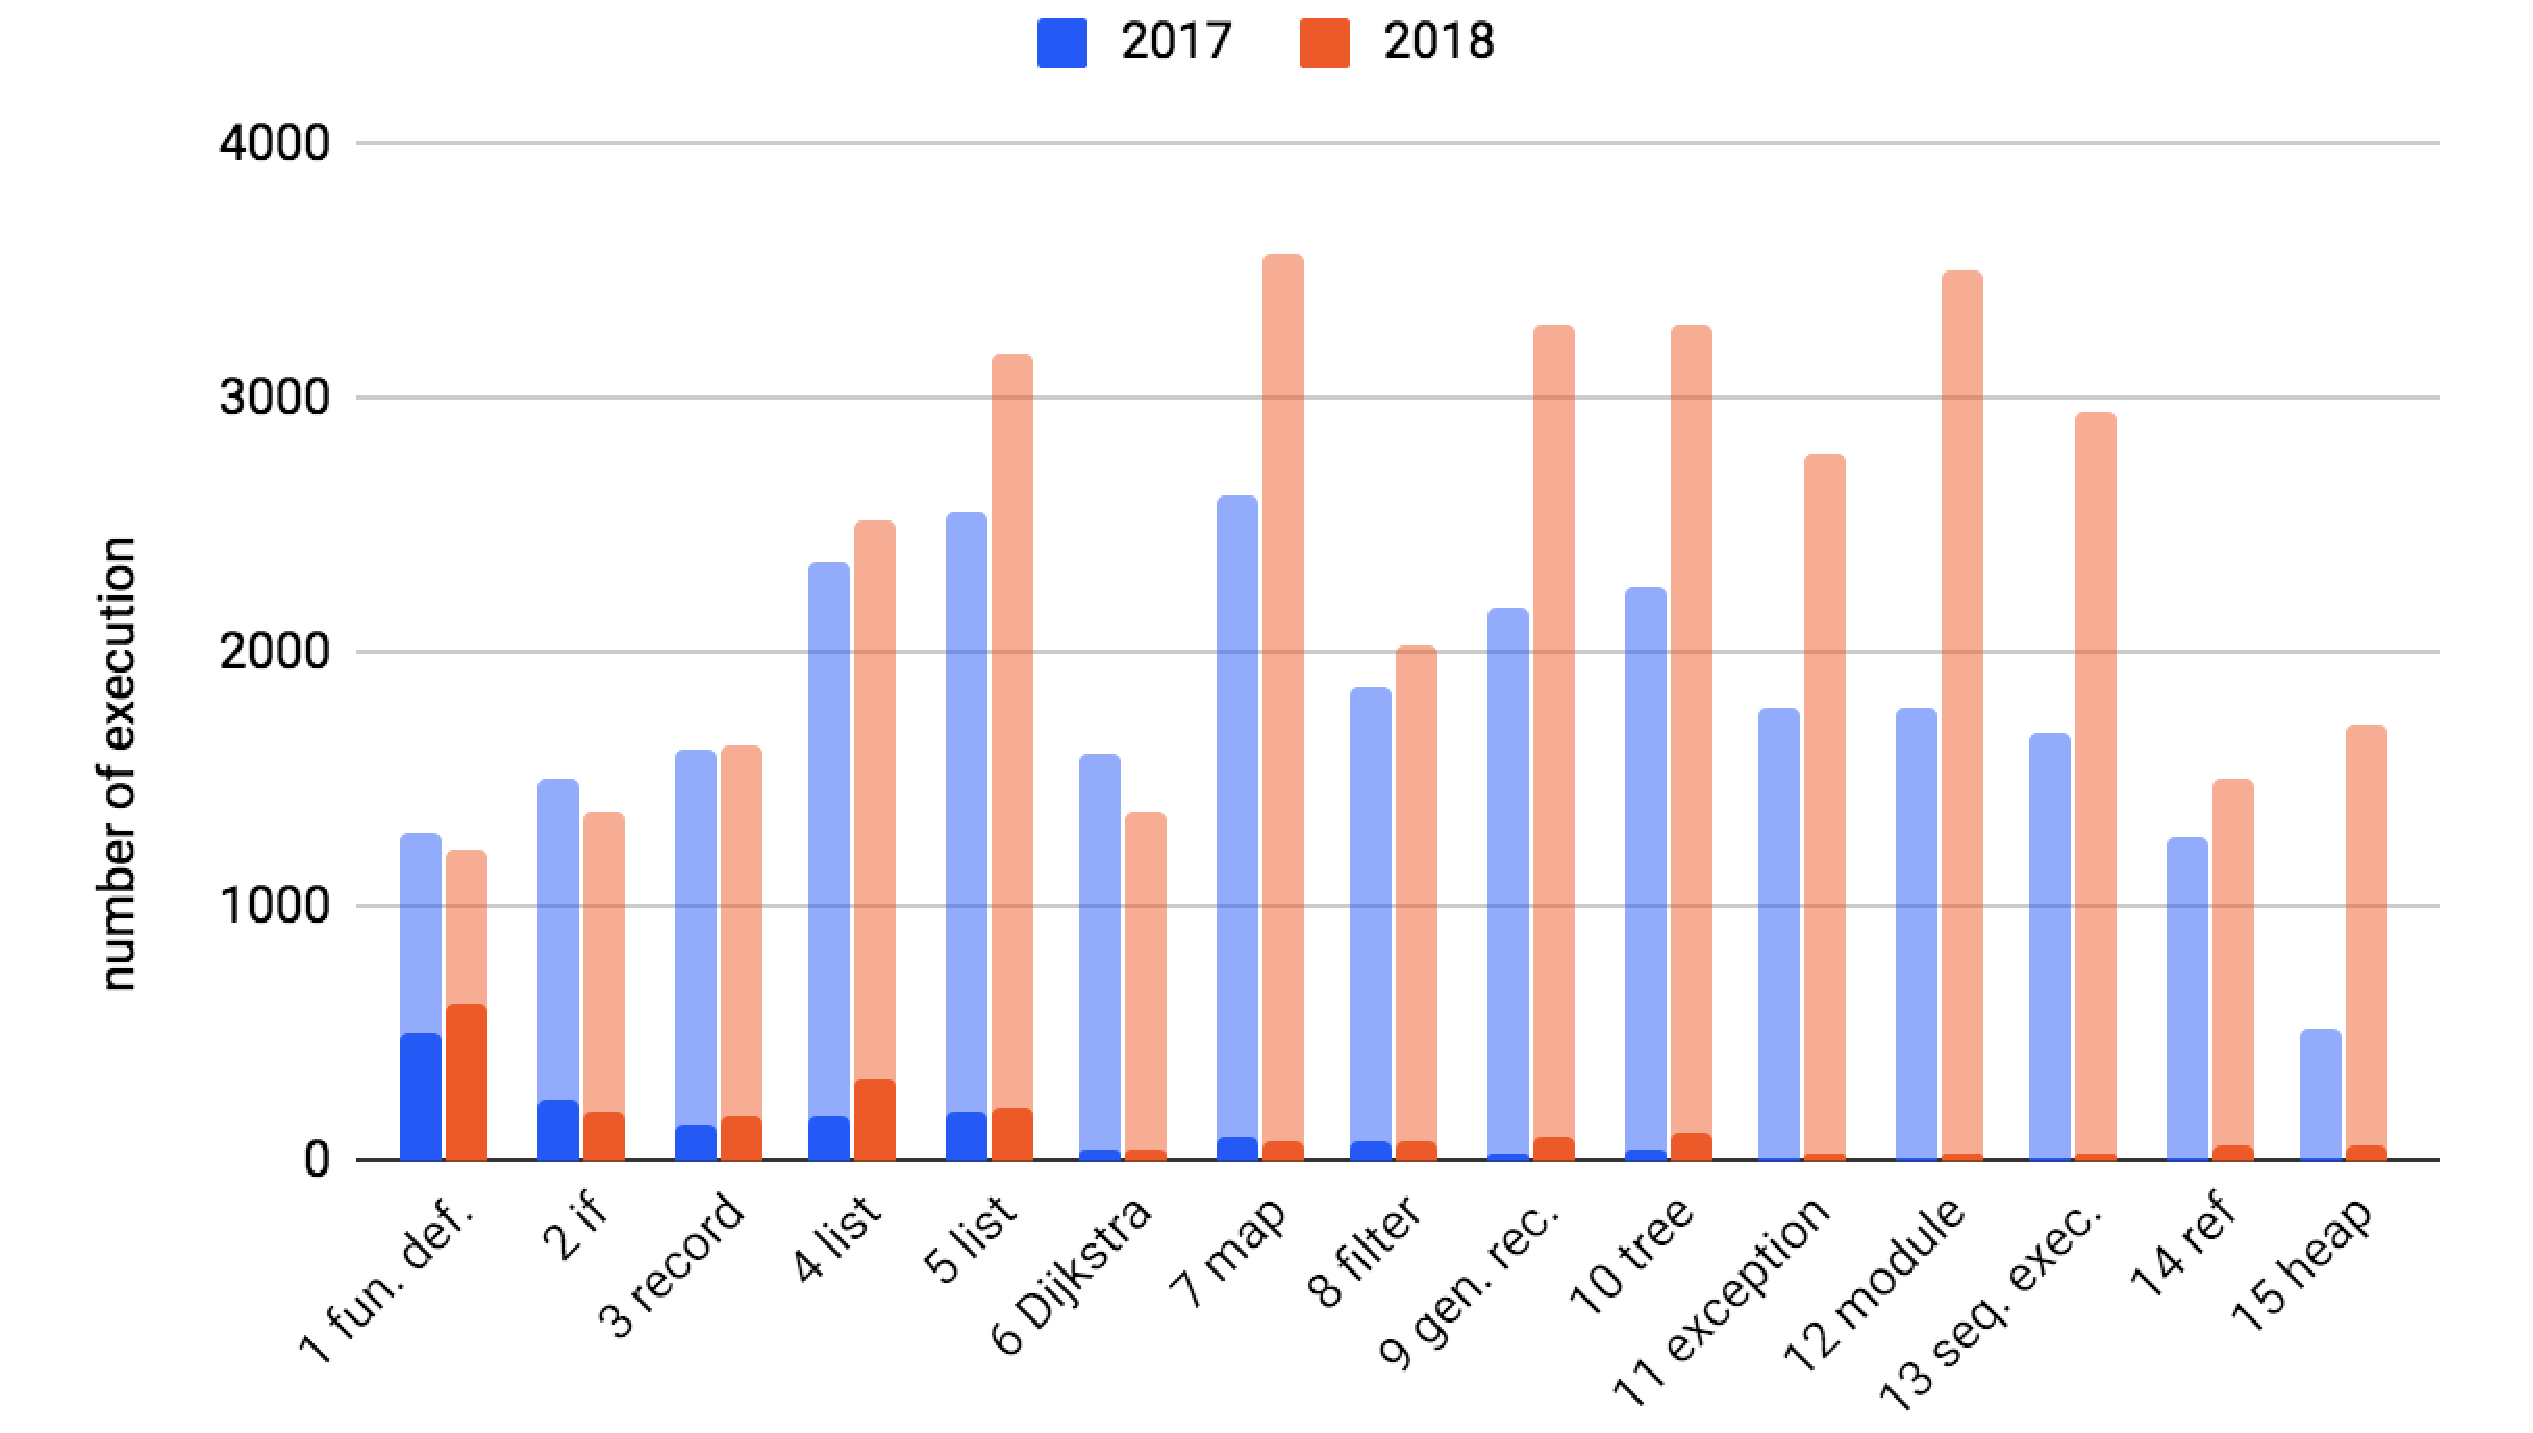
\includegraphics[width=15cm]{6/table1a.eps}
    \caption{Frequency of standard execution (light-colored) and step execution (dark-colored) in each week in 2017 and 2018. The stepper was not used at all toward the end of the course in 2017, but it was used in some degree in 2018.}
    \label{figure:allExecution}
  \end{center}
\end{figure}

\begin{figure}[!t]
  \begin{center}
    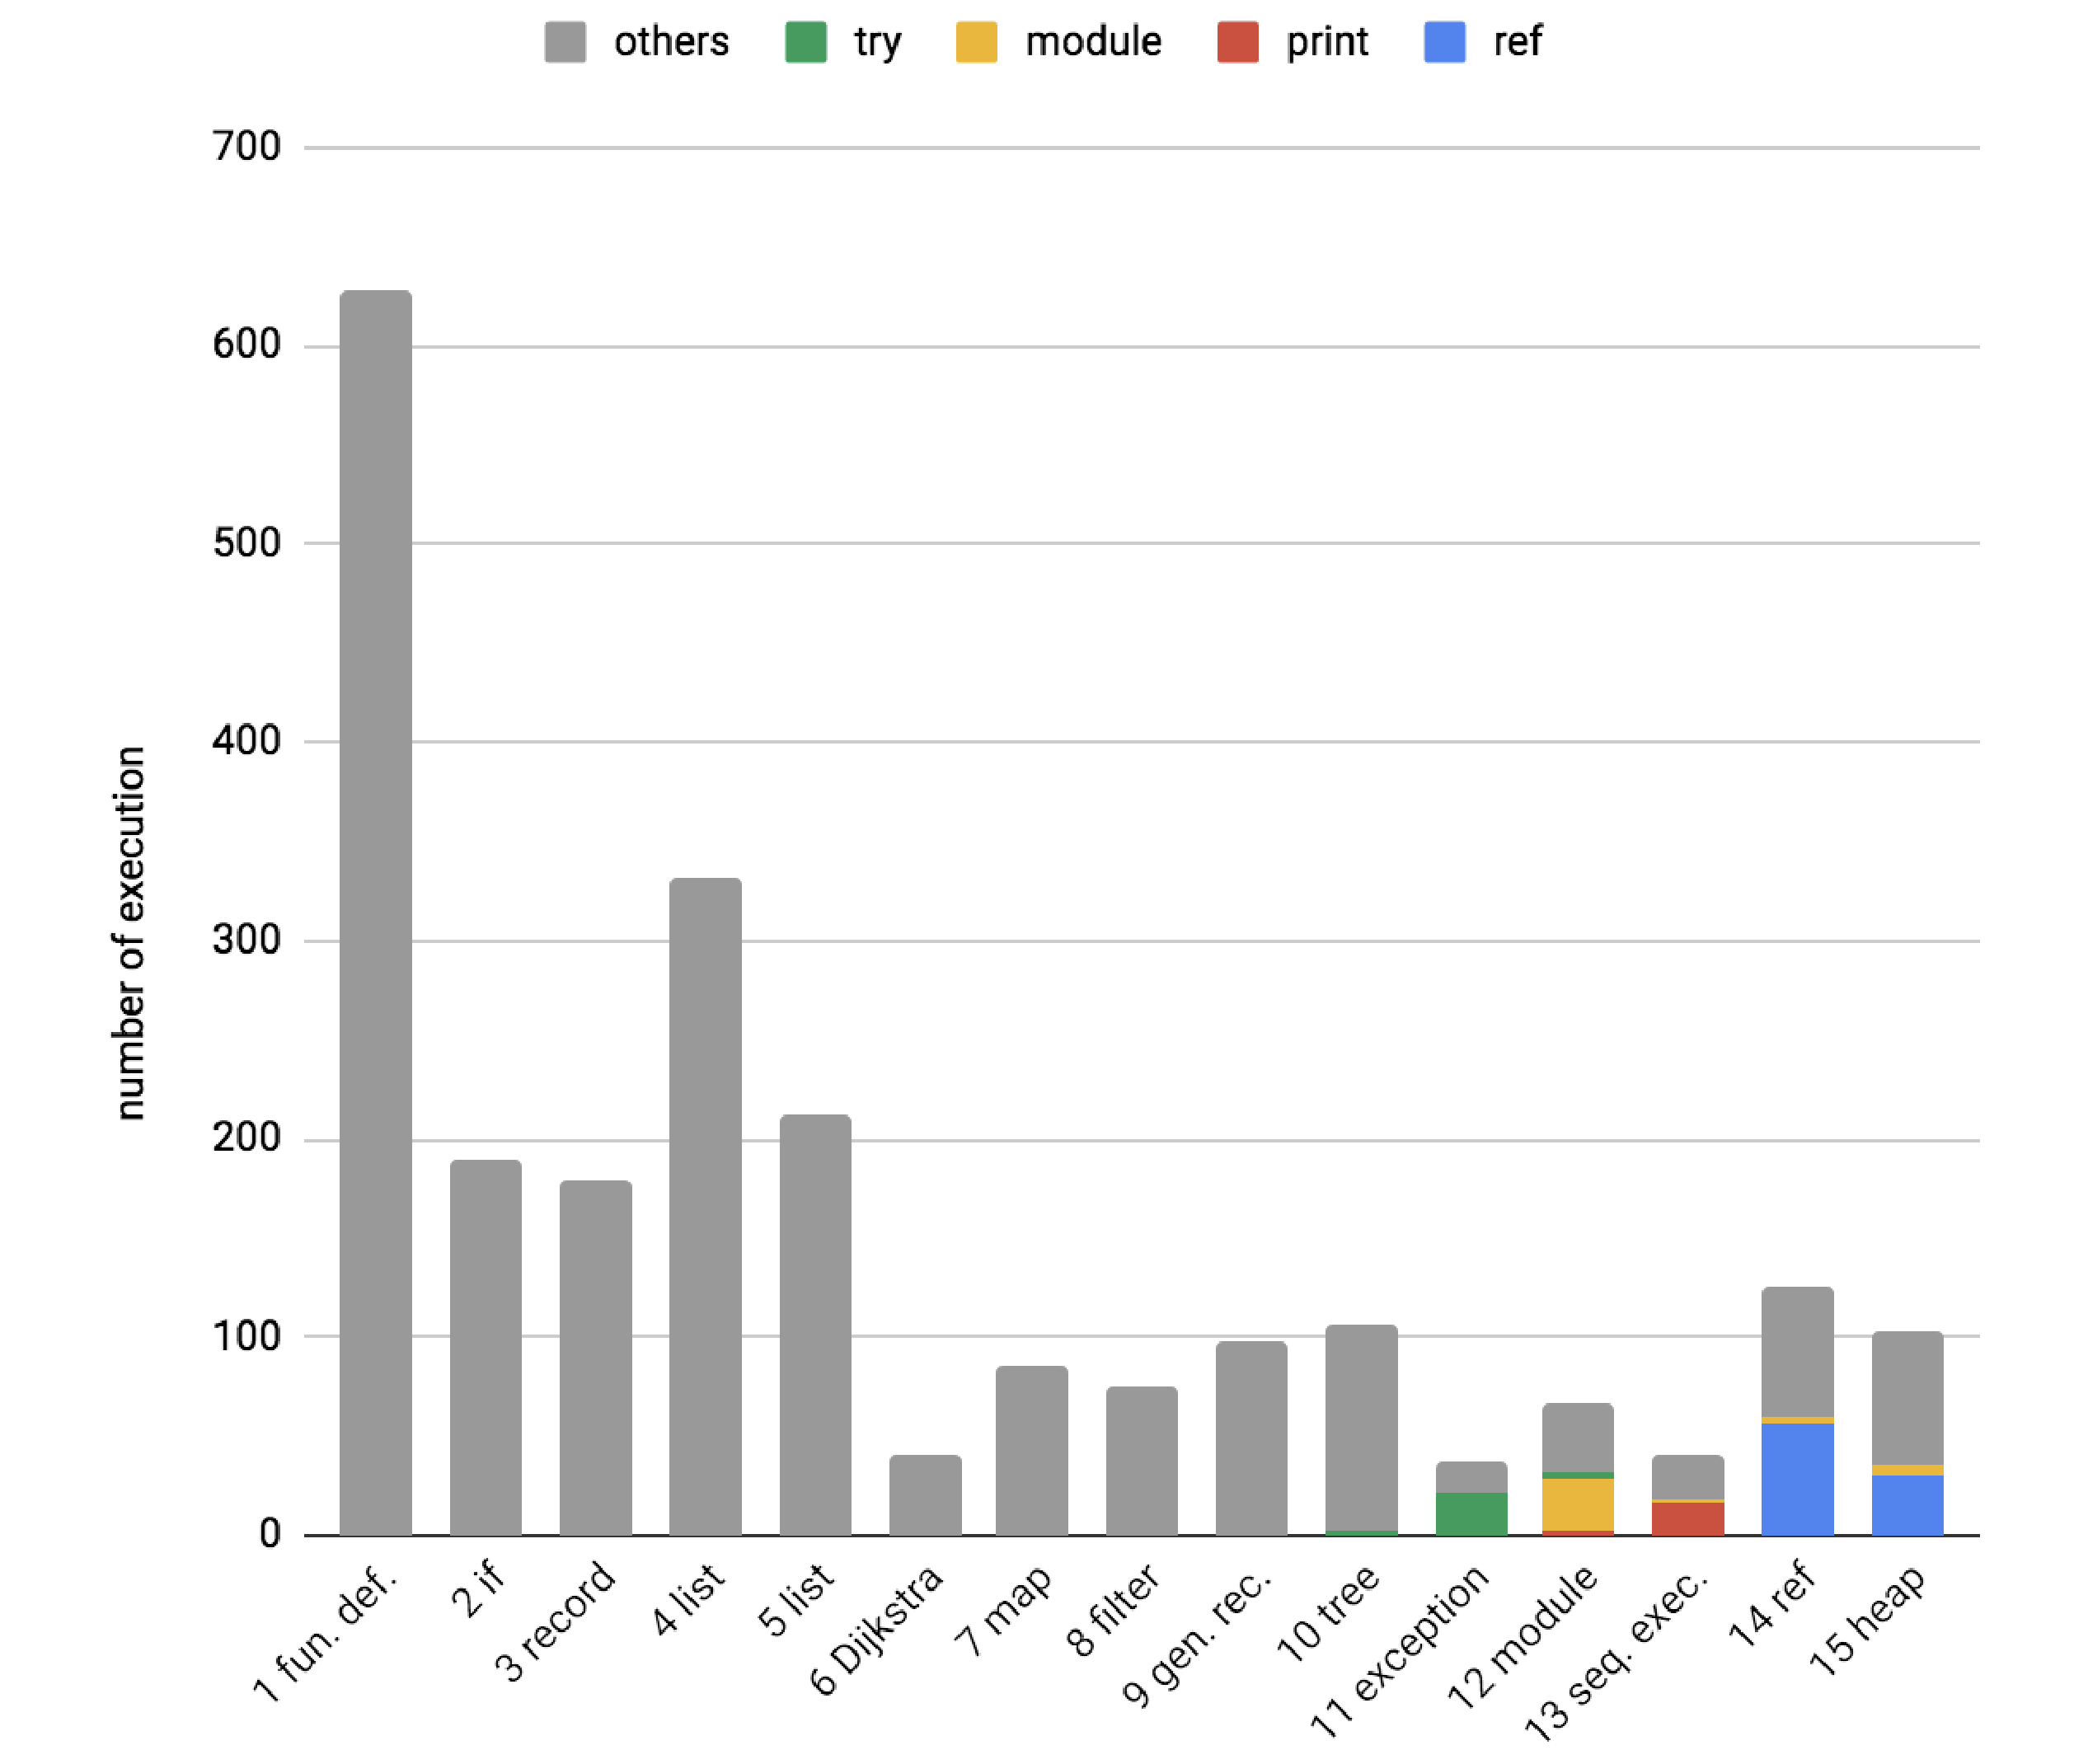
\includegraphics[width=15cm]{6/table1b.eps}
    \caption{Number of times the stepper was used to evaluate a program with ``try'', ``module'', ``print'' or ``ref'' in 2018.}
    \label{figure:stepExecution}
  \end{center}
\end{figure}

Figure \ref{figure:allExecution} shows how many times students used the stepper among all the executions including the ones that ended up in an error.
%% Table~\ref{TableUsage} shows how many times students used the stepper
%% (the column ``step.'') among all the executions (``all'') including the
%% ones that ended up in an error.
%% The table further shows a breakdown of the step-executed programs.
In both 2017 and 2018, the stepper was used quite often until week 5.
This is partly because
we encouraged students to use the stepper when they had
trouble finding bugs and understanding recursion.
After week 5, the number decreases, because students started using an
interpreter, too, as programs became larger.

In 2017, the number of stepper uses decreases toward the end of the
course.
In contrast, in 2018, certain number of stepper uses is observed,
thanks to the support of exception handling, modules, and references.
Figure \ref{figure:stepExecution} shows the number of execution of programs using these features during step-execution in 2018. % 足した execution を単数にした
From the figure, we can see that there is a demand for step
%% From the table, we observe that some students try to see step
execution of advanced constructs such as exception handling and
modules.

The exact numbers of execution are available in Table \ref{TableUsage} in the Appendix.
%% These graphs were generated from Table \ref{TableUsage} of the Appendix.

\subsection{Effects of Stepper}
It is not easy to see the effect of a tool like a stepper on
the learning of students.
In the case of improving error messages of a compiler, for example,
one can classify various errors and see how many of them are covered
by the improved error messages objectively.
For the stepper, it is unclear how to show such numeric data.

\begin{figure}
  \begin{center}
    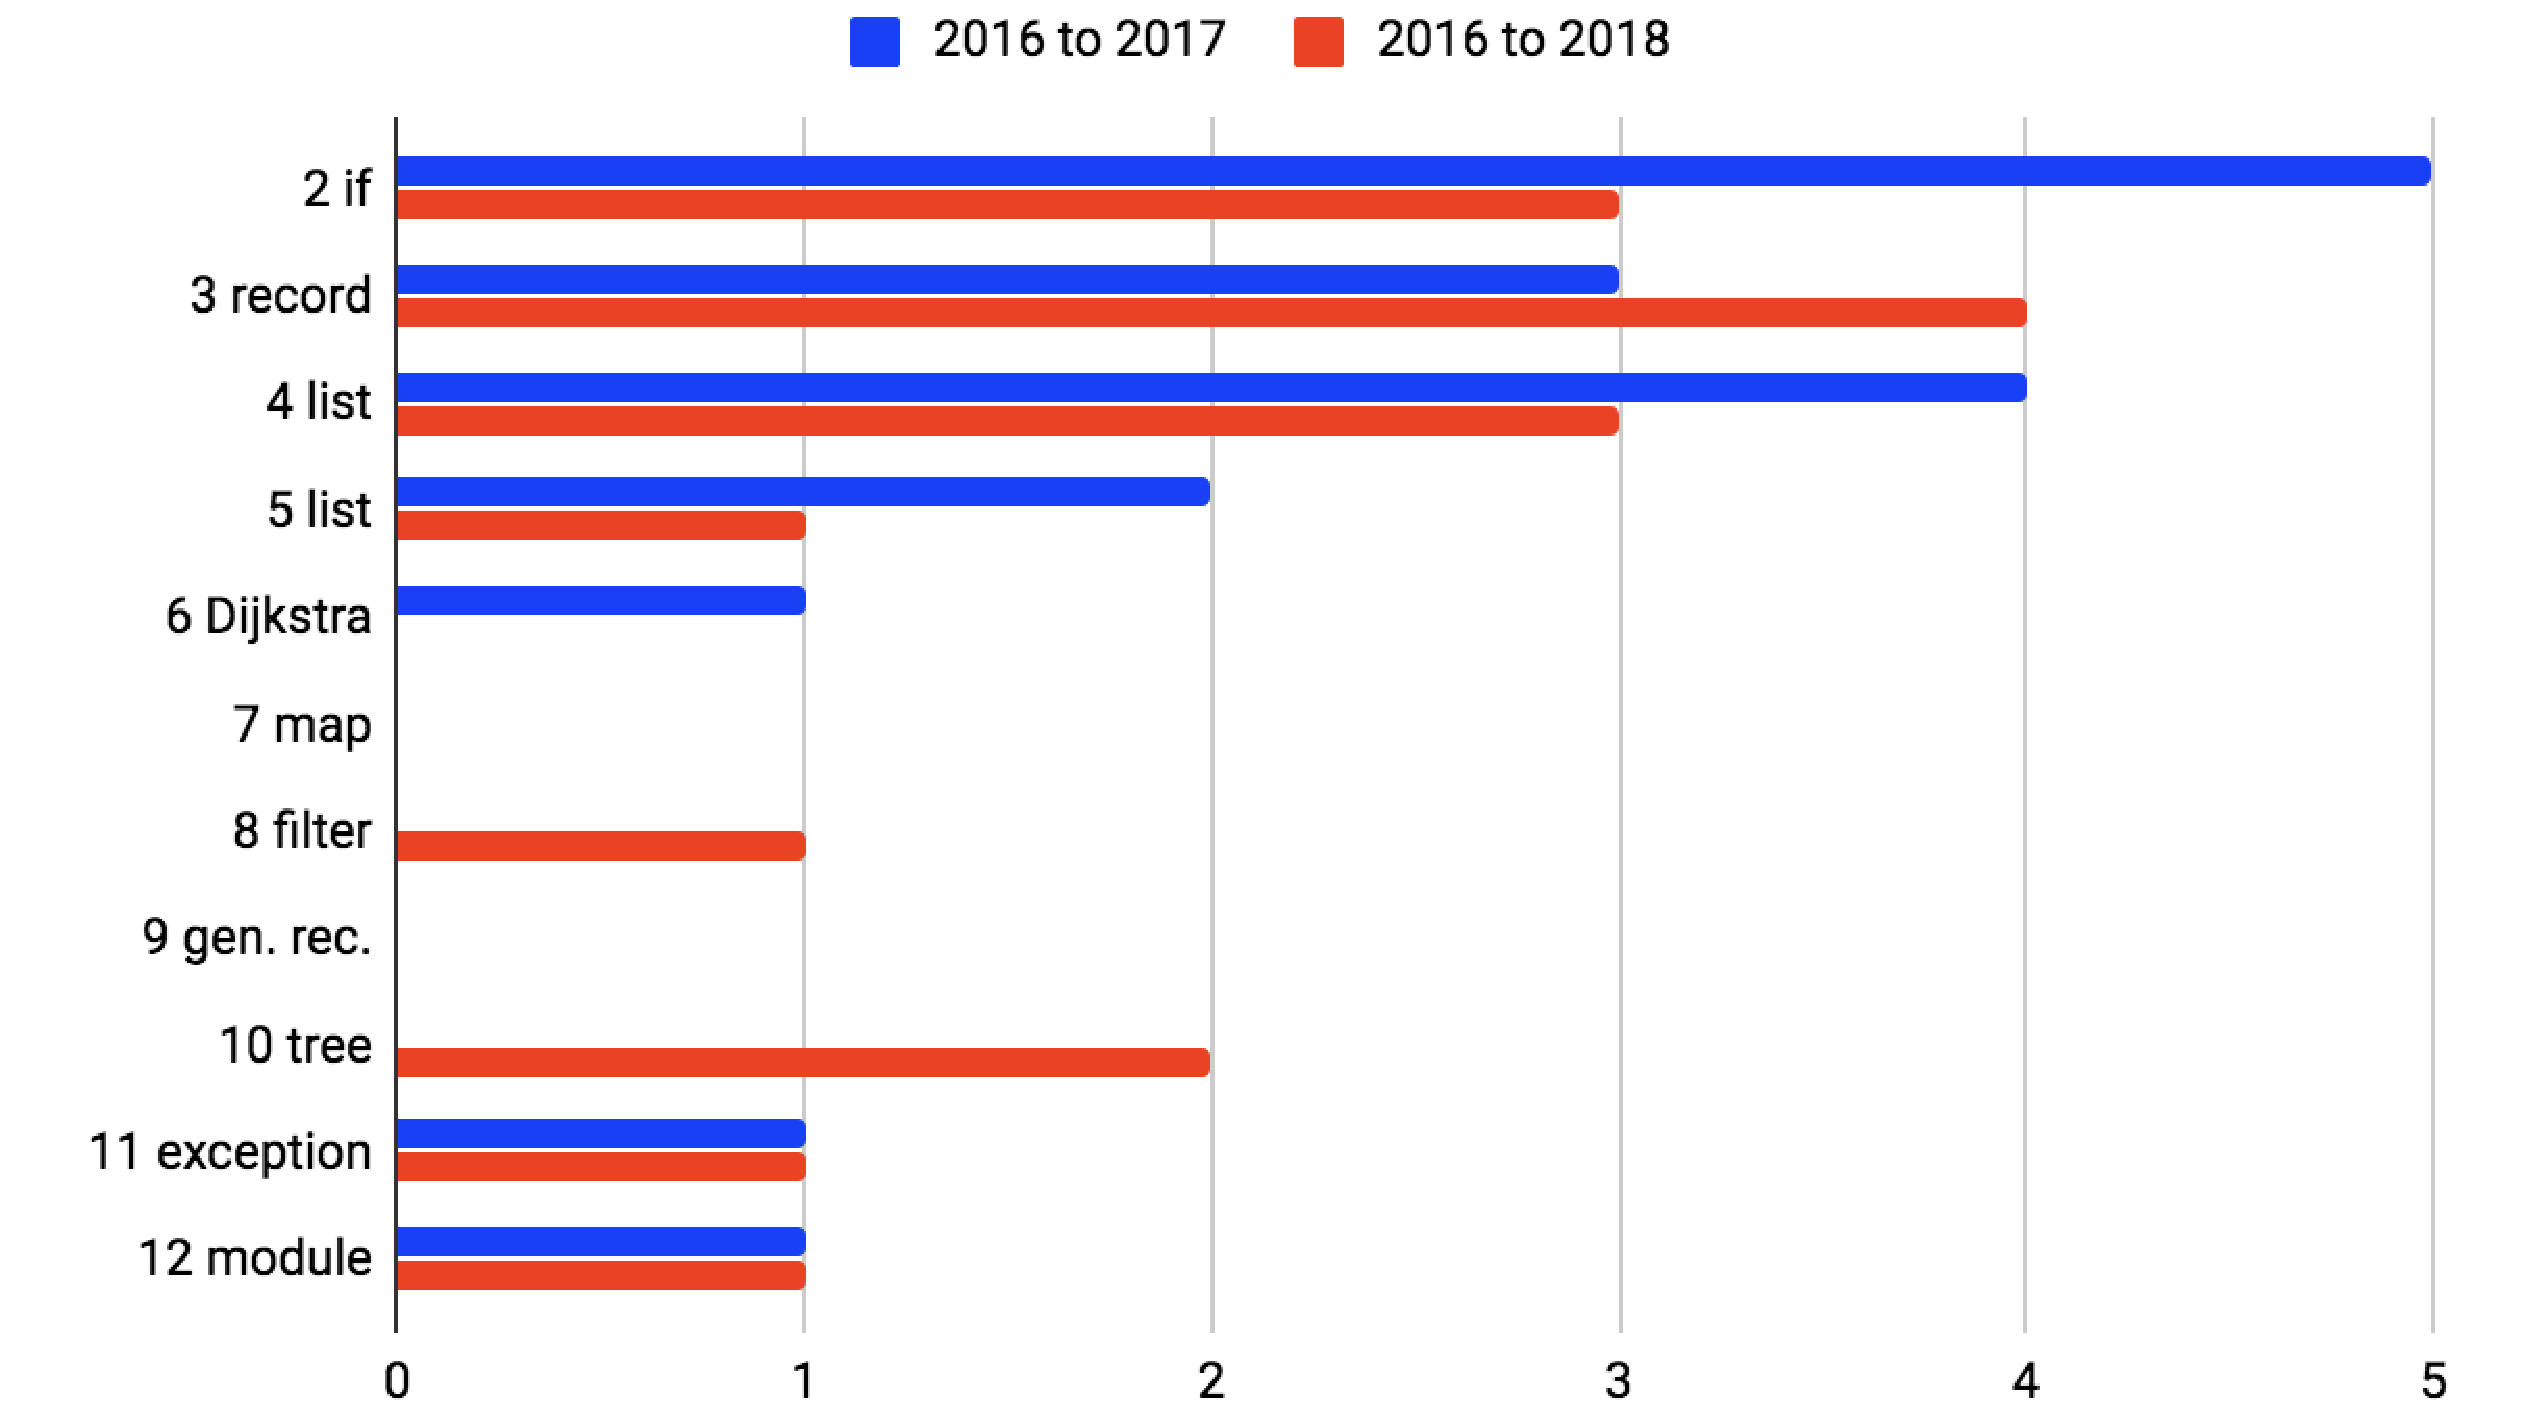
\includegraphics[width=15cm]{6/table2.eps}
    \caption{Number of questions where students arrived at a correct answer significantly faster in 2017 and 2018 than 2016.}
    \label{figure:p}
  \end{center}
\end{figure}

As an attempt to measure the effect of the stepper, we examined how
long students took to submit correct solutions to the check system.
Among all the submitted correct solutions, we gathered the (wall-clock) times of
submissions recorded in the check system that are within 100 minutes
from the beginning of the class and compared the average times among
2016, 2017, and 2018.
%% Table~\ref{TableTTest} shows the result.

Figure \ref{figure:p} shows the number of questions for which students submitted a correct answer within significantly shorter time in 2017 and 2018 compared to 2016.  The data are based on one-sided t-testing with p-value $< 0.05$; we refer the reader to Table \ref{TableTTest} of the appendix for details.
Note that we did not include week 1 because we had a special pre-test in the first lecture in 2018.
%% For all the problems from week 2 to week 12 (the last week where the
%% check system is available), the average time of correct submissions in
%% 2018 is compared to that of 2016 and 2017.
%% We did not include week 1, because we had a special pre-test in the
%% first lecture in 2018.
%% The problem numbers that start with ‘r’ are for practice problems, which are mostly solved in the day of the lecture. The ones without are report problems, some of which are difficult and are solved only later in the week.
%% The figure shows how many questions students submitted correct answers in 2017 or 2018 significantly earlier than in 2016 for each lecture, based on one-sided t-testing with p-value $<0.05$ (Detailed values are listed in Table \ref{TableUsage} in the appendix) .
%% The table shows the result of one-sided t-testing with p-values,
%% whether the use of the stepper in 2017 and 2018 makes the average time
%% earlier than in 2016.

From the figure, we can see improvement of submission times after the (real) introduction of the stepper, especially in earlier problems.
%% From the figure, we observe that for both 2017 and 2018, the average
%% times of correct solutions for many problems (in particular, the easier
%% ones) are significantly earlier than 2016.
However, there is an exception: for one problem in the 6th week, correct submissions come significantly later in 2018 than in 2016.
%% One exception is for the problem 6.r1 in 2018.
%% For this problem, the average time for 2018 is significantly later
%% than 2016.
The problem simply asks students to write a recursive function that adds 1 to each
element of a given list.
We do not know why it took so long in 2018.
The result of t-testing all the problems together is t(1778) = 2.819 (p=0.002) in 2017 and t(2111) = 2.592 (p=0.005) in 2018.
%% The last row shows the result of t-testing all the problems together,
%% which shows the same trend as most of the problems.
%% This could be partly attributed to the uses of the stepper for better
%% understanding the behavior of programs.

We also compared the average times between 2017 and 2018.
For earlier weeks (up to week 5), submissions in 2017 were
significantly earlier, while for later weeks,
there were no significant difference
(except for two problems where the average
times for 2018 were earlier).
Putting all the problems together, the two were not significantly
different with t(1953)=0.455 (p=0.324).

\paragraph{Threats to validity.}
It is possible that the results of our experiment were affected by the enrolled students in each year (there was no over-lapping).
In all the three years, 
the instructor started the class with some introductory comments that
vary in length.
Although the instructor made similar comments in each year, they were
not exactly the same, which could have affected.

\subsection{Students' Evaluation}

\begin{table}
  \begin{center}
  \begin{tabular}{|l|c|r|}
    \hline
    & score & \# of students \\ \hline
    Using the stepper, I could almost always understand & & \\
    the behavior of programs or the cause of errors. & 4 & 3 \\ \hline
    Using the stepper, I could often solve problems at hand. & 3 & 8\\ \hline
    Using the stepper, I could sometimes solve problems at hand. & 2 & 25\\ \hline
    I could rarely find new things using the stepper. & 1 & 2\\ \hline
    The stepper was useless.  I did not use the stepper. & 0 & 0\\ \hline
%   4 & ステッパを使えばほぼ必ずプログラムの動きや間違いの原因が分かった & 3\\ \hline
%   3 & ステッパを使って問題を解決できることが多くあった & 8\\ \hline
%   2 & たまにステッパを使って問題を解決できることがあった & 25\\ \hline
%   1 & ステッパを使うことで新たに何かが分かることはほとんど無かった & 2\\ \hline
%   0 & 全く役に立たなかった、または使わなかった & 0\\ \hline
  \end{tabular}
  \end{center}
  \caption{Students' scoring of the stepper in 2018.
  38 students out of 42 answered.
  The average is 2.3.}
% 平均 2.3158、38 / 42 人が回答
  \label{TableScore}
\end{table}

At the end of the semester of 2018, we asked the students to share
their thoughts on the stepper.
We received responses from 38 out of 42 students.
We first asked whether the stepper was useful on the 0 to 4 point scale.
The results, which we present in Table \ref{TableScore}, suggest
that the stepper is not a silver bullet that is useful
for all the time.
However, most students could solve the problems at hand sometimes
using the stepper.
We are encouraged to see some students choose ``the stepper was almost always useful''.

We next asked students to write when the stepper was useful (if any),
such as when they found their misunderstanding, or when they could
deepen their understanding.
We summarize the answers in two categories.

\paragraph{Understanding of the behavior of programs.}
Seven students answered they could deepen their understanding of
the behavior of programs.
In particular, five students among them wrote explicitly that the
stepper helped them figure out how functions consume recursive data.
We imagine it was particularly instructive to see how a recursive 
function definition is unfolded in nesting application.
% TODO: この文の意味が不明

Other students answered that they could observe the behavior of
programs in general.
They found that arguments of a function are evaluated before the
function call, and that the elements of a list are evaluated one by one.
Among them, one student observed the right-to-left execution
employed in OCaml.
Previously, such subtle behavior was taught only in passing without
much emphasis.

\paragraph{Debugging.}
Many students found the stepper useful for debugging.
Sixteen students answered they could find what was wrong when their
program did not pass test cases.
By observing each step of execution, they could identify when the
program behaved differently from their expectation.
This is an important step toward debugging in general.
Because printing (and side effects) is handled at the end of the
course, the only debugging method for students had been unit testing:
they checked whether all the component functions worked as expected.
With the stepper, they can simply observe execution of the program and
see when it goes wrong.

Three students found the stepper useful to understand why their
program did not terminate.
Without printing, it is not easy for students to identify the cause of
infinite loops.
Using the stepper, one of the students could not only observe
the infinite loop, but also see how far her program went well
and when it went wrong.
